\section{Training on the missing scattering structures}
\label{sec:adaptation}
The earlier equation model had no training examples from the nonplanar box, pentagon or box with external virtuality. To test whether training on these structures helps, we fit a new seed tree and equation tree for each structure. We preserve the original models and their tests. Appendix~\ref{app:models} defines the new labels and models.

The study uses separate training, validation and test batches. Table~\ref{tab:scattering-split} gives their sizes. Rational batches use different invariant values in each split. Symbolic batches keep all independent invariants symbolic and use disjoint target lists within the symbolic split. The graph structures are shared across splits, so this tests adaptation within these structures.

\begin{table}[!htbp]
\centering\small
\caption{The additional scattering study. Each of the three structures contributes equally to the batch counts.}
\label{tab:scattering-split}
\begin{tabular}{@{}lrrr@{}}\toprule
Part & Rational batches & Symbolic batches & Targets\\\midrule
Training & 6 & 3 & 108\\
Validation & 3 & 3 & 60\\
Testing & 6 & 3 & 108\\\bottomrule
\end{tabular}
\end{table}

Each tree has maximum depth twelve. The seed trees use sixteen features and assign the same score to all operators of a seed. The equation trees use seventeen features, including the operator index. Kira enumerates its usual seed region, and the selected model filters equations before coefficient construction. Both methods preserve native elimination. These are new tree models fitted on native reductions; the original neural networks remain unchanged.

Validation compares three score thresholds and fixes the best setting before testing. The test compares native choices, the original equation tree, the new seed tree and the new equation tree on identical targets. It includes prediction, exact algebra, coefficient checks, cleanup and fallback. Reference discovery, training and later record archiving remain outside the timer. Five repetitions give 180 test calculations. Separate applications receive a master basis without access to target reference coefficients, and their returned coefficients are checked afterward.



The new fit uses 59,706 equation records and 4,674 grouped seed records. These counts include repeated candidate patterns in different training batches. Table~\ref{tab:scattering-fit} gives the sizes of the fitted trees. No test record enters these fits.

\begin{table}[!htbp]
\centering\small
\caption{Additional training records and tree sizes. Each graph uses three training batches.}
\label{tab:scattering-fit}
\begin{tabular}{@{}lrrrr@{}}\toprule
Structure & Seed records & Seed nodes & Equation records & Equation nodes\\\midrule
Nonplanar box & 4,326 & 67 & 56,238 & 819 \\
Pentagon & 258 & 15 & 2,838 & 179 \\
Box with virtuality & 90 & 11 & 630 & 81 \\
\bottomrule
\end{tabular}
\end{table}

All 180 test calculations pass exact coefficient checks, covering 9,880 returned coefficient entries. All eighteen basis-only applications also pass their separate coefficient checks. Each new selector completes all 45 first attempts without fallback. The original equation model requires fallback in all 45 trials on these same new test cases.

Removing fallback improves the learned methods relative to the original filter, but does not establish a saving against native Kira. The new seed model's full-time ratio is $1.027$, with descriptive 95\% interval $[0.995,1.086]$. The new equation model's ratio is $1.017$, with interval $[0.988,1.054]$. Their measured average times are therefore 2.7\% and 1.7\% higher than native time. The original filter's ratio on this new test is $1.368$, or 36.8\% more time. This differs from the earlier 25.2\% result because the parameter points and symbolic targets differ.

\begin{table}[!htbp]
\centering\small
\caption{New reserved test results. Each value uses five repetitions. Ratios divide model time by native time; values below one are faster.}
\label{tab:scattering-time}
\begin{tabular}{@{}lrrrr@{}}\toprule
Case & Native (s) & Original tree & New seeds & New equations\\\midrule
Nonplanar box (13) & 4.163 & 1.293 & 1.023 & 0.980 \\
Nonplanar box (14) & 4.140 & 1.221 & 1.002 & 0.974 \\
Nonplanar box (symbolic) & 4.458 & 1.233 & 0.983 & 1.010 \\
Pentagon (13) & 1.005 & 1.439 & 0.963 & 1.016 \\
Pentagon (14) & 0.965 & 1.436 & 1.069 & 1.038 \\
Pentagon (symbolic) & 1.120 & 1.356 & 0.958 & 0.979 \\
Box with virtuality (13) & 0.826 & 1.339 & 0.953 & 0.991 \\
Box with virtuality (14) & 0.763 & 1.529 & 1.152 & 1.124 \\
Box with virtuality (symbolic) & 0.729 & 1.499 & 1.166 & 1.052 \\
\midrule
Geometric mean ratio & --- & 1.368 & 1.027 & 1.017\\\bottomrule
\end{tabular}
\end{table}

Table~\ref{tab:scattering-time} and Figures~\ref{fig:adapted-time}--\ref{fig:adapted-sufficiency} show the distinction between enough equations and faster reduction. Some cases become faster and others become slower. We keep native choices as the application default for these scattering cases because the reserved test gives no reliable overall saving. The trained models remain available for further comparisons.

The result supports adding examples from the missing structures to improve equation sufficiency. It does not prove that missing data were the only cause of the original failure. This study also fits separate trees for each graph and changes the seed-model architecture. It tests adaptation within three structures, rather than transfer to arbitrary new graphs or higher loops. The timing intervals resample the three graph groups and describe this small comparison. They do not establish performance over all scattering integrals.

\begin{figure}[tbp]
\centering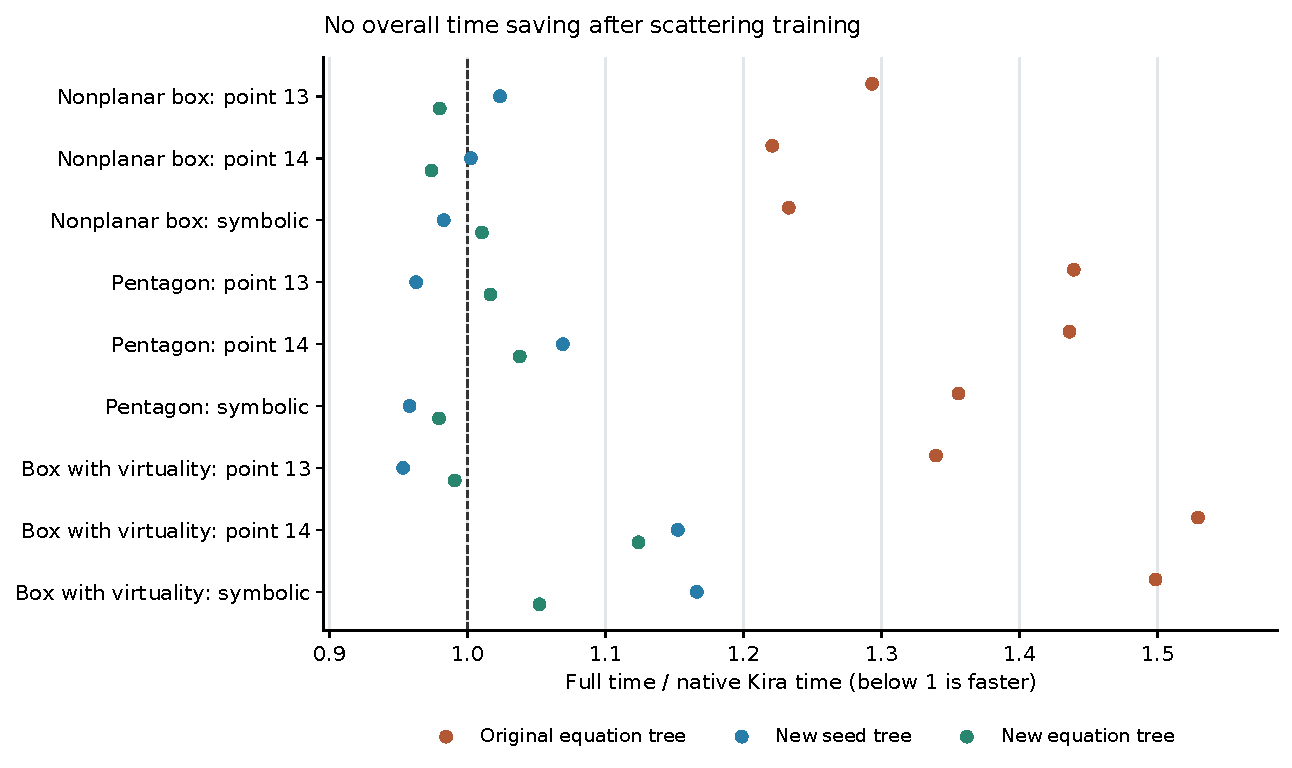
\includegraphics[width=\linewidth]{paper_figures/scattering_training.pdf}
\caption{Training on the three structures removes much of the original filter's overhead, but gives no overall saving against native Kira. Points compare five-run median full times, including prediction, checks and fallback. The dashed line marks equal time. No per-case uncertainty interval is inferred from five repetitions.}
\label{fig:adapted-time}
\end{figure}

\begin{figure}[tbp]
\centering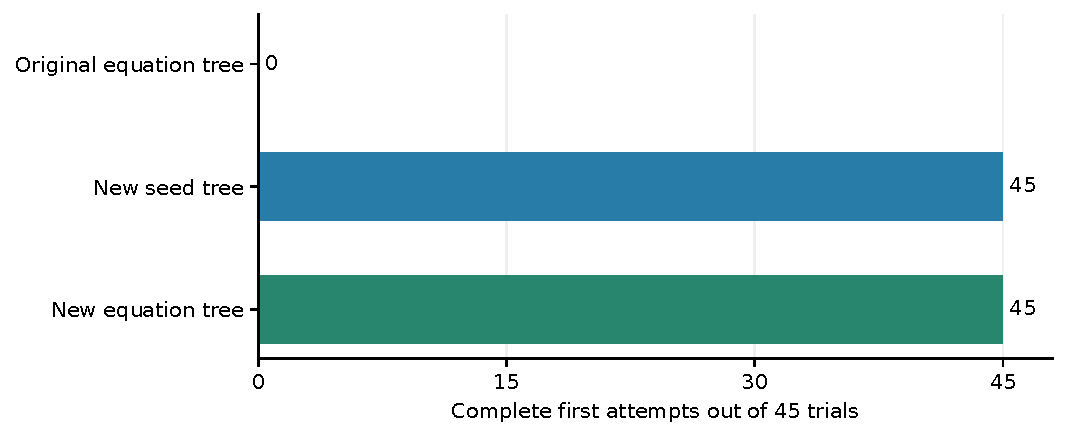
\includegraphics[width=.85\linewidth]{paper_figures/scattering_sufficiency.pdf}
\caption{The new selectors provide sufficient equations on every first attempt. Each method has 45 trials across nine batches. Native fallback lets the original filter eventually complete, and its added time remains in the comparison above.}
\label{fig:adapted-sufficiency}
\end{figure}
\FloatBarrier
